\documentclass[10pt,a4paper]{report}

% Caricamento dei 3 pacchetti condivisi dalla radice
\usepackage{../pacchetti}
\usepackage{../box-colori}
\usepackage{../comandi}

% Intestazioni e piè di pagina
\pagestyle{fancy}
\fancyhf{}
\fancyhead[L]{\textcolor{bluscuro}{\textbf{Dispensa di Telecomunicazioni -- Classe 2 TELQ}}}
\fancyhead[R]{\textcolor{bluscuro}{Prof. Bernardis Pierluigi}}
\fancyfoot[C]{\thepage}

\renewcommand{\chaptermark}[1]{\markboth{\thechapter.\ #1}{}}
\renewcommand{\sectionmark}[1]{\markright{\thesection\ #1}}

% Dati del documento
\title{\Huge{\textcolor{bluscuro}{Dispensa di Telecomunicazioni}}}
\author{Prof. Bernardis Pierluigi\\ Classe 2 TELQ}
\date{A.S. 2026/2027}

\setcounter{tocdepth}{1}

\begin{document}

\maketitle
\tableofcontents

% primo_capitolo.tex

\chapter{Carica, campo e grandezze elettriche}

\begin{concetto}
Questo capitolo introduce i concetti fondamentali dell'elettricità: la carica elettrica, la forza di Coulomb, il campo elettrico, il lavoro elettrico, la tensione, la corrente e la resistenza. L'obiettivo è costruire un percorso coerente che parta dalla proprietà più elementare della materia (la carica) e arrivi alle grandezze che si misurano ogni giorno in laboratorio.
\end{concetto}

\section{La carica elettrica}


La \textbf{carica elettrica} è una proprietà intrinseca della materia, esattamente come la massa. Questo significa che non è qualcosa che si aggiunge dall'esterno: è una caratteristica che i corpi possiedono per il solo fatto di essere fatti di materia. Non è possibile però darne una definizione diretta, nel senso che non possiamo dire ``la carica è\dots'' indicando qualcosa di visibile o toccabile. Possiamo soltanto \textbf{osservarne gli effetti}: attrazione, repulsione, scintille, corrente elettrica, campi elettrici. La carica, in altre parole, la conosciamo attraverso i fenomeni che produce.

La carica elettrica si misura in \textbf{coulomb} [\(\text{C}\)]. Si tratta di un'unità di misura piuttosto grande per gli standard quotidiani: la carica che si accumula strofinando un palloncino è di qualche miliardesimo di coulomb.

\subsection{Le particelle subatomiche}

Per capire da dove viene la carica elettrica bisogna guardare dentro la materia. La materia è fatta di atomi, e ogni atomo è formato da particelle più piccole. Le tre particelle che ci interessano sono:

\begin{concetto}
\textbf{Le particelle che portano la carica}
\begin{itemize}[leftmargin=1cm]
  \item i \textbf{protoni}, che si trovano nel nucleo dell'atomo e possiedono \textbf{carica positiva};
  \item i \textbf{neutroni}, anch'essi nel nucleo, che \textbf{non possiedono carica};
  \item gli \textbf{elettroni}, che orbitano attorno al nucleo e possiedono \textbf{carica negativa}.
\end{itemize}
La carica del protone e quella dell'elettrone hanno lo stesso valore assoluto, ma segno opposto. Il neutrone è elettricamente neutro, cioè non ha carica.
\end{concetto}

Il valore assoluto della carica elementare, indicato con \(e\), è
\[
e = 1{,}602 \times 10^{-19}\,[\text{C}].
\]
Poiché ogni corpo è fatto di atomi, e ogni atomo contiene un numero intero di protoni ed elettroni, la carica elettrica totale di un corpo è sempre un multiplo intero di \(e\):
\[
Q = \pm n\,e, \qquad n \in \mathbb{N}.
\]

In condizioni normali un corpo è \textbf{elettricamente neutro}: ha tanti protoni quanti elettroni, e le cariche positive e negative si bilanciano. Se però riusciamo a spostare qualche elettrone da un corpo a un altro, i due corpi acquistano una carica netta.

\begin{esempio}
\textbf{L'esperimento del palloncino.} Si strofina un palloncino di gomma sui capelli. Durante lo strofinamento, alcuni elettroni passano dai capelli al palloncino. Alla fine:
\begin{itemize}[leftmargin=1cm]
  \item il palloncino ha più elettroni che protoni, quindi possiede una \textbf{carica negativa};
  \item i capelli hanno perso elettroni, quindi possiedono una \textbf{carica positiva}.
\end{itemize}
Se ora si avvicina il palloncino a un muro, esso vi aderisce: la carica negativa del palloncino respinge gli elettroni presenti sulla superficie del muro, lasciando esposta una zona con carica positiva che attira il palloncino. Lo stesso fenomeno si osserva avvicinando il palloncino a dei piccoli pezzetti di carta, che vengono attratti.
\end{esempio}

\begin{concetto}
\textbf{Regola generale.} Cariche dello stesso segno si respingono; cariche di segno opposto si attraggono. Questa regola è alla base di tutti i fenomeni elettrici.
\end{concetto}


\section{La forza di Coulomb}


Tra due corpi carichi si esercita una forza. Il fisico francese Charles-Augustin de Coulomb, alla fine del Settecento, stabilì sperimentalmente che questa forza ha un'espressione molto semplice. Se si considerano due cariche puntiformi \(Q_1\) e \(Q_2\) poste a distanza \(r\), il modulo della forza è
\[
F = k\,\frac{Q_1\,Q_2}{r^2},
\]
dove \(k\) è la costante di coulomb che dipende dal mezzo in cui si trovano le cariche. Nel vuoto vale
\[
k = 8{,}99 \times 10^9\,\left[\frac{\text{N}\cdot\text{m}^2}{\text{C}^2}\right].
\]

La forza agisce lungo la retta che congiunge le due cariche: questa retta si chiama \textbf{congiungente}. La direzione della forza è quindi sempre quella della congiungente, mentre il verso dipende dal segno delle cariche.

\begin{concetto}
\textbf{Analisi della formula.} La forza di Coulomb ha tre proprietà fondamentali:
\begin{itemize}[leftmargin=1cm]
  \item è \textbf{direttamente proporzionale} al prodotto delle cariche: se una delle due cariche raddoppia, la forza raddoppia; se raddoppiano entrambe, la forza quadruplica;
  \item è \textbf{inversamente proporzionale al quadrato della distanza}: se la distanza raddoppia, la forza diventa un quarto; se triplica, diventa un nono;
  \item ha \textbf{segno} che dipende dal prodotto \(Q_1 Q_2\): se le cariche sono concordi la forza è positiva (repulsiva), se sono discordi è negativa (attrattiva).
\end{itemize}
\end{concetto}



\subsection{L'analisi dimensionale della costante \(k\)}

Possiamo ricavare le unità di misura di \(k\) a partire dalla legge di Coulomb. Scriviamo la formula del modulo
\[
F = k\,\frac{Q_1\,Q_2}{r^2}
\]
e sostituiamo le unità di misura di ciascuna grandezza:
\[
[\text{N}] = [k] \cdot \frac{[\text{C}] \cdot [\text{C}]}{[\text{m}]^2}.
\]
Isolando \([k]\) si ottiene
\[
[k] = \frac{[\text{N}] \cdot [\text{m}]^2}{[\text{C}]^2}.
\]
Questa è l'unità di misura della costante di Coulomb nel Sistema Internazionale. Esprimendo il newton come chilogrammo per metro su secondo quadro, si ha anche
\[
[k] = \frac{[\text{kg}] \cdot [\text{m}]^3}{[\text{s}]^2 \cdot [\text{C}]^2}.
\]

\begin{curiosita}
L'analisi dimensionale non serve solo a scrivere correttamente le unità di misura, ma anche a controllare la coerenza di una formula. Se da un calcolo risultasse un'unità di misura diversa da quella attesa, ci sarebbe sicuramente un errore da qualche parte.
\end{curiosita}

\section{Il campo elettrico}


Quando due cariche interagiscono, si può pensare che la forza si eserciti ``a distanza'', cioè senza che ci sia nulla in mezzo. In realtà il modo moderno di descrivere questa interazione è diverso: si dice che una carica \textbf{modifica lo spazio} attorno a sé, creando un \textbf{campo elettrico}. Una seconda carica posta in quel punto risente del campo e quindi di una forza.

Il campo elettrico è una grandezza \textbf{vettoriale} e si indica con \(\vec{E}\). Esso descrive l'effetto che una configurazione di cariche produce in ogni punto dello spazio, indipendentemente dal fatto che in quel punto ci sia o meno una carica che lo subisce.

\subsection{Definizione operativa}

Per definire il campo elettrico in un punto si utilizza una \textbf{carica di prova}, cioè una carica piccolissima (in modo che non disturbi la configurazione delle cariche che generano il campo) e positiva (per convenzione). Se in un punto dello spazio si pone una carica di prova \(q_0\) e questa risente di una forza \(\vec{F}\), il campo elettrico in quel punto è definito come
\[
\vec{E} = \frac{\vec{F}}{q_0}.
\]
Il campo elettrico è quindi la \textbf{forza per unità di carica}. La sua unità di misura è il newton su coulomb:
\[
[\text{E}] = \frac{[\text{N}]}{[\text{C}]} = \left[\frac{\text{N}}{\text{C}}\right].
\]

\begin{concetto}
Il campo elettrico è definito come rapporto tra la forza di Coulomb che agisce su una carica di prova \(q_0\) e la carica di prova stessa. Il campo non dipende da \(q_0\), ma solo dalla configurazione di cariche che lo genera. Cambiando la carica di prova, la forza cambia in proporzione, ma il loro rapporto rimane costante.
\end{concetto}

\subsection{Il campo di una carica puntiforme}

Se la carica che genera il campo è una carica puntiforme \(Q\), e la carica di prova \(q_0\) si trova a distanza \(r\) da essa, la forza di Coulomb vale
\[
F = k\,\frac{Q\,q_0}{r^2}.
\]
Dividendo per \(q_0\) si ottiene il modulo del campo elettrico:
\[
E = \frac{F}{q_0} = k\,\frac{Q}{r^2}.
\]
Il campo elettrico di una carica puntiforme è quindi direttamente proporzionale alla carica che lo genera e inversamente proporzionale al quadrato della distanza.

\subsection{Campo di corpi positivi e negativi}


\begin{concetto}
\textbf{Linee di campo di una carica puntiforme}
\begin{itemize}[leftmargin=1cm]
  \item se \(Q\) è \textbf{positiva}, il campo elettrico punta \textbf{verso l'esterno}: le linee di campo escono dalla carica e si allontanano da essa;
  \item se \(Q\) è \textbf{negativa}, il campo elettrico punta \textbf{verso l'interno}: le linee di campo entrano nella carica.
\end{itemize}
Il campo elettrico è sempre diretto lungo la congiungente tra la carica che lo genera e il punto in cui si misura.
\end{concetto}

\begin{figure}[htbp]
\centering
\begin{tikzpicture}[scale=0.9]
% Carica positiva
\filldraw[fill=red!30, draw=red!70!black] (-3,0) circle (0.15);
\foreach \ang in {0,30,...,330} {
  \draw[-{Stealth[length=2mm]}, thick, bluscuro]
    ({-3+0.3*cos(\ang)}, {0.3*sin(\ang)}) --
    ({-3+1.2*cos(\ang)}, {1.2*sin(\ang)});
}
\node[align=center] at (-3,-1.8) {Campo di una carica\\ positiva};

% Carica negativa
\filldraw[fill=blue!30, draw=blue!70!black] (3,0) circle (0.15);
\foreach \ang in {0,30,...,330} {
  \draw[-{Stealth[length=2mm]}, thick, bluscuro]
    ({3+1.2*cos(\ang)}, {1.2*sin(\ang)}) --
    ({3+0.3*cos(\ang)}, {0.3*sin(\ang)});
}
\node[align=center] at (3,-1.8) {Campo di una carica\\ negativa};
\end{tikzpicture}
\end{figure}



\begin{esempio}
\textbf{Il campo elettrico e il campo gravitazionale.}

La Terra ha una massa enorme e, per questo, \textbf{genera attorno a sé un campo gravitazionale}. In ogni punto dello spazio vicino alla Terra, un oggetto lasciato libero risente di una forza diretta verso il centro della Terra. Questo campo esiste indipendentemente dal fatto che ci sia qualcuno a sentirlo: esiste perché c'è la Terra.\\

Ora immagina di voler \textbf{misurare} il campo gravitazionale in un punto vicino alla superficie terrestre. Per farlo, potresti prendere un oggetto e lasciarlo cadere. Ma attenzione: se prendessi un oggetto enorme, come una seconda Luna, la sua stessa massa modificherebbe il campo gravitazionale terrestre nel punto in cui la metti. Il campo che misureresti non sarebbe più quello della Terra da sola, ma quello della Terra \emph{più} l'oggetto che hai aggiunto. Non avresti misurato il campo della Terra: avresti misurato un campo diverso.\\

Per questo, per misurare il campo gravitazionale della Terra, si prende un oggetto \textbf{piccolissimo}, una persona per esempio. La sua massa è così piccola che la sua presenza \textbf{non modifica il campo gravitazionale della Terra}. Il campo che si misura è quindi davvero quello generato dalla Terra, non quello di un sistema Terra-persona.\\

Questo è esattamente lo stesso ragionamento che si fa con il campo elettrico:

\begin{itemize}[leftmargin=1cm]
  \item La \textbf{Terra} è come la carica \(Q\) che genera il campo;
  \item il \textbf{campo gravitazionale} della Terra è come il \textbf{campo elettrico} \(\vec{E}\) generato da \(Q\);
  \item la \textbf{persona} è come la \textbf{carica di prova} \(q_0\);
  \item la \textbf{forza} che la persona sente cadendo è come la \textbf{forza elettrica} \(\vec{F}\) che agisce sulla carica di prova.
\end{itemize}

La persona deve essere piccolissima, altrimenti modificherebbe il campo che vogliamo misurare. Allo stesso modo, la carica di prova \(q_0\) deve essere piccolissima, altrimenti la sua presenza altererebbe la configurazione delle cariche che generano il campo. Solo così possiamo dire di aver misurato il campo \emph{generato da \(Q\)}, e non un campo modificato dalla carica di prova stessa.\\

Ed è per questo che il campo elettrico, definito come \(\vec{E} = \frac{\vec{F}}{q_0}\), \textbf{non dipende da \(q_0\)}: se la carica di prova raddoppia, la forza raddoppia, ma il loro rapporto resta lo stesso. Il campo è una proprietà del punto dello spazio, non della carica che vi si mette dentro.
\end{esempio}




\section{Lavoro di una forza e lavoro elettrico}


Prima di parlare di lavoro elettrico, è necessario ricordare che cosa si intende, in fisica, per \textbf{lavoro}. Si consideri una forza costante \(\vec{F}\) applicata a un corpo che si sposta di un tratto \(s\) lungo la direzione della forza. Si definisce \textbf{lavoro} il prodotto
\[
L = F \cdot s,
\]
dove \(F\) è il modulo della forza e \(s\) è il modulo dello spostamento. Il lavoro si misura in \textbf{joule} [\(\text{J}\)].

Se la forza e lo spostamento hanno la stessa direzione e lo stesso verso, il lavoro è positivo: la forza ``aiuta'' il movimento. Se hanno verso opposto, il lavoro è negativo: la forza ``si oppone'' al movimento. Se la forza è perpendicolare allo spostamento, il lavoro è nullo.

\begin{esempio}
    Il lavoro che compie la forza di gravità su un corpo che cade è positivo: la forza di gravità aiuta il corpo a muoversi e gli trasferisce energia.\\
    Il lavoro che compie la forza di attrito su un corpo che scivola su un piano inclinato è negativo: la forza di attrito si oppone al movimento e sottrae energia al corpo.\\
    Il lavoro che compie la forza di gravità su un corpo che si muove in orizzontale è nullo: la forza di gravità è perpendicolare allo spostamento e non trasferisce energia al corpo.
\end{esempio}


\begin{concetto}
Il lavoro è il modo con cui una forza trasferisce energia a un corpo. Un lavoro positivo aumenta l'energia del corpo; un lavoro negativo la diminuisce; un lavoro nullo non la modifica.
\end{concetto}

\subsection{Il lavoro elettrico}

Nel caso della forza elettrica, il lavoro compiuto dalla forza di Coulomb su una carica che si sposta da un punto A a un punto B si chiama \textbf{lavoro elettrico}. Se la forza elettrica che agisce sulla carica è \(\vec{F}_e = Q\,\vec{E}\), e la carica si sposta di un tratto \(s\) lungo la direzione del campo, il lavoro elettrico è:
\[
L_e = F_e \cdot s = Q\,E\,s.
\]
Il lavoro elettrico si misura anch'esso in \textbf{joule} [\(\text{J}\)].

\begin{esempio}
\textbf{Carica positiva che si muove nel verso del campo.} Una carica positiva \(Q > 0\) posta in un campo elettrico \(\vec{E}\) risente di una forza \(\vec{F}_e\) nello stesso verso del campo. Se la carica si sposta nel verso del campo, il lavoro elettrico è positivo: la forza elettrica aiuta la carica a muoversi e le trasferisce energia.
\end{esempio}

\begin{esempio}
\textbf{Carica negativa che si muove nel verso del campo.} Una carica negativa \(Q < 0\) posta nello stesso campo elettrico risente invece di una forza \textbf{opposta} al campo. Se la carica si sposta nel verso del campo, il lavoro elettrico è negativo: la forza elettrica si oppone al movimento.
\end{esempio}

\section{La tensione elettrica}

A partire dal lavoro elettrico si può definire una grandezza molto importante: la \textbf{tensione elettrica}, o \textbf{differenza di potenziale}. La tensione tra due punti A e B di un circuito è definita come il \textbf{lavoro elettrico per unità di carica} compiuto per spostare una carica da A a B:
\[
V_{AB} = \frac{L_e}{Q}.
\]
La tensione si misura in \textbf{volt} [\(\text{V}\)], e vale la relazione
\[
1\,[\text{V}] = 1\,\left[\frac{\text{J}}{\text{C}}\right].
\]
In altre parole, se per spostare una carica di \(1\,\text{C}\) da A a B il campo elettrico compie un lavoro di \(1\,\text{J}\), allora la tensione tra A e B è di \(1\,\text{V}\).

\begin{concetto}
\textbf{Interpretazione fisica.} La tensione è la ``spinta'' che il campo elettrico esercita su ogni unità di carica. È una proprietà della coppia di punti A e B, non della carica che si sposta: se la carica raddoppia, il lavoro raddoppia, ma il loro rapporto rimane invariato.
\end{concetto}

\begin{esempio}
\textbf{La tensione di una pila.} Una pila stilo ha una tensione di circa \(1{,}5\,\text{V}\). Questo significa che, per spostare una carica di \(1\,\text{C}\) dal polo negativo al polo positivo all'interno della pila, il campo elettrico compie un lavoro di \(1{,}5\,\text{J}\). La pila è quindi un dispositivo che mantiene una differenza di potenziale tra i suoi due terminali.
\end{esempio}

\subsection{La tensione non dipende dal percorso}

La tensione è stata definita come lavoro elettrico per unità di carica. A questo punto sorge spontanea una domanda: se il lavoro dipendesse dal percorso scelto per andare da A a B, anche la tensione ne dipenderebbe, e non avrebbe senso parlare di ``tensione tra due punti''. Per fortuna, la forza elettrica ha una proprietà molto importante: il lavoro che essa compie non dipende dal percorso, ma solo dal punto di partenza e dal punto di arrivo.

Per capire questo concetto, si consideri un campo elettrico uniforme, per esempio quello che si crea tra due piastre piane parallele cariche di segno opposto. In un campo uniforme, il campo elettrico ha lo stesso modulo, la stessa direzione e lo stesso verso in tutti i punti. Si supponga di voler spostare una carica \(Q\) da un punto A a un punto B, e di poter scegliere tra due percorsi diversi.

\begin{figure}[htbp]
\centering
\begin{tikzpicture}[scale=1]
  % Piastre
  \draw[thick, fill=red!10] (-3,3) -- (3,3) -- (3,3.5) -- (-3,3.5) -- cycle;
  \draw[thick, fill=blue!10] (-3,-3) -- (3,-3) -- (3,-3.5) -- (-3,-3.5) -- cycle;
  \node[right] at (-3,3.25) {+  +  +  +  +  +  +  +  +  +  +  +  +  +  +};

    \foreach \i [evaluate=\i as \x using (-3 + (\i-1)*(6/14)*1.06)] in {1,...,13} {
    \node[right] at (\x,-3.25){\(-\)};
  }

  % Linee di campo
  \foreach \x in {-2.5,-1.5,-0.5,0.5,1.5,2.5} {
    \draw[-{Stealth[length=2mm]}, gray] (\x,2.8) -- (\x,-2.8);
  }

  % Percorso 1: dritto
  \draw[very thick, rossoscuro, -{Stealth[length=3mm]}] (-2,2) -- (-2,-2);
  \node[left, rossoscuro] at (-2.2,1.5) {Percorso 1};

  % Percorso 2: a zig-zag (spezzata)
  \draw[very thick, verdescuro, -{Stealth[length=3mm]}]
    (-2,2) -- (0,2) -- (0,0) -- (2,0) -- (2,-2) -- (-2, -2);
  \node[above, verdescuro] at (0.5,2.1) {Percorso 2};

  % Punti A e B
  \filldraw (-2,2) circle (0.08) node[above left] {A};
  \filldraw (-2,-2) circle (0.08) node[below left] {B};
\end{tikzpicture}
\end{figure}

Lungo il \textbf{Percorso 1}, la carica si muove parallelamente al campo. Poiché la forza elettrica è diretta lungo il campo, in ogni tratto la forza e lo spostamento sono paralleli e concordi. Il lavoro totale è
\[
L_1 = Q \cdot E \cdot d,
\]
dove \(d\) è la distanza tra A e B lungo la direzione del campo.

Lungo il \textbf{Percorso 2}, la carica si muove prima perpendicolarmente al campo, poi parallelamente, poi di nuovo perpendicolarmente. Nei tratti perpendicolari, la forza elettrica è perpendicolare allo spostamento, quindi il lavoro compiuto è nullo. Solo nel tratto parallelo il lavoro è diverso da zero, e vale ancora \(Q \cdot E \cdot d\). Di conseguenza
\[
L_2 = Q \cdot E \cdot d = L_1.
\]

Qualunque percorso si scelga, spezzandolo in tanti piccoli tratti paralleli e perpendicolari al campo, si ottiene sempre lo stesso risultato: il lavoro dipende solo dalla componente dello spostamento lungo la direzione del campo, cioè dalla ``differenza di quota elettrica'' tra A e B. I tratti perpendicolari non contribuiscono al lavoro, quelli paralleli si sommano algebricamente.

\begin{concetto}
\textbf{La tensione non dipende dal percorso.} Il lavoro elettrico compiuto per spostare una carica da un punto A a un punto B dipende solo dai due punti, non dal cammino seguito. Di conseguenza, anche la tensione \(V_{AB} = \frac{L_e}{Q}\) dipende solo da A e B, e non dal percorso. Questa proprietà si esprime dicendo che \textbf{la forza elettrica è conservativa}.
\end{concetto}

\begin{esempio}
\textbf{Il paragone con la forza peso.} Immagina di dover portare una valigia dal primo piano al terzo piano di un palazzo. Puoi salire dritto per le scale, oppure fare un giro tortuoso passando per altri piani. Il lavoro compiuto contro la forza di gravità è sempre lo stesso, perché dipende solo dal dislivello tra il punto di partenza e quello di arrivo.
\end{esempio}

\begin{concetto}
\textbf{Il filo conta solo per quello che collega.} Nei circuiti ideali, il filo che collega due punti ha una forma che non conta nulla: potrebbe essere dritto, attorcigliato su se stesso, cortissimo o lunghissimo, passare da una parte o dall'altra del circuito. Quello che conta, e che determina i calcoli, è soltanto \textbf{tra quali punti} il filo è collegato. La tensione tra due punti di un circuito è sempre la stessa, indipendentemente da come sono fisicamente collegati. Per questo motivo, nei disegni dei circuiti, i fili si rappresentano sempre come segmenti dritti e puliti: la forma è solo una comodità grafica, non ha alcun significato elettrico.
\end{concetto}

\section{La corrente elettrica}


La \textbf{corrente elettrica} è un flusso ordinato di cariche elettriche che si muovono tutte nella stessa direzione. Per quantificarla si introduce una grandezza che misura ``quanta carica passa attraverso una sezione del conduttore nell'unità di tempo''. Questa grandezza si chiama \textbf{intensità di corrente} e si indica con \(I\).

La corrente è definita come il rapporto tra la carica \(\Delta Q\) che attraversa una sezione del conduttore e l'intervallo di tempo \(\Delta t\) in cui avviene il passaggio:
\[
I = \frac{\Delta Q}{\Delta t}.
\]
L'intensità di corrente si misura in \textbf{ampere} [\(\text{A}\)], e vale la relazione
\[
1\,[\text{A}] = 1\,\left[\frac{\text{C}}{\text{s}}\right].
\]
Da questa definizione si ricavano immediatamente le due formule inverse:
\[
\Delta Q = I \cdot \Delta t, \qquad \Delta t = \frac{\Delta Q}{I}.
\]

\begin{concetto}
\textbf{Verso convenzionale della corrente.} Per ragioni storiche, il verso convenzionale della corrente è quello che va dal polo positivo al polo negativo, anche se in realtà gli elettroni si muovono in senso opposto. Questa convenzione è ancora oggi universalmente accettata.
\end{concetto}

\begin{esempio}
\textbf{Valori tipici di corrente}
\begin{itemize}[leftmargin=1cm]
  \item lampadina di una torcia: circa \(0{,}3\,[\text{A}]\);
  \item caricabatterie di un telefonino: circa \(1\,[\text{A}]\);
  \item forno elettrico: circa \(10\,[\text{A}]\);
  \item fulmine: fino a \(30\,000\,[\text{A}]\), per un tempo brevissimo.
\end{itemize}
\end{esempio}

\section{Leggi di Ohm}


\subsubsection{L'esperimento di Ohm}

Georg Simon Ohm, all'inizio del XIX secolo, si pose una domanda semplice: \emph{come varia la corrente che attraversa un conduttore al variare della tensione applicata ai suoi capi?} Per rispondere, utilizzò un \textbf{provino cilindrico}, cioè un filo conduttore di forma cilindrica, di lunghezza \(l\) e sezione \(S\) note, collegato a un generatore di tensione variabile.

Lo schema dell'esperimento è il seguente:
\begin{itemize}[leftmargin=1cm]
  \item un \textbf{generatore di tensione variabile} applica ai capi del provino una tensione \(V\), che può essere cambiata a piacere, rappresentata nel circuito seguente con una batteria;
  \item un \textbf{voltmetro} misura la tensione \(V\) ai capi del provino;
  \item un \textbf{amperometro} misura la corrente \(I\) che lo attraversa.
\end{itemize}





\begin{figure}[htbp]
  \centering
  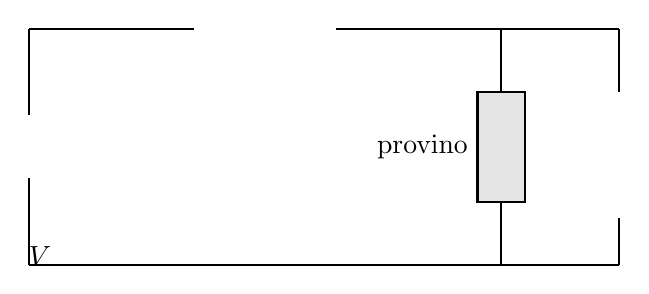
\begin{tikzpicture}
    % Usa il comando senza graffe extra in coda
    

    % Istruzioni TikZ terminate correttamente da punto e virgola
    \draw[thick, fill=gray!20] (5.7,0.8) rectangle (6.3,2.2);
    \node[left] at (5.7,1.5) {provino};
    \voltmetro[label={voltmetro}, label x=1.3, label y=0.05]{7.5}{1.5}

    \draw[thick] (0, 1.9) -- (0, 3);
    \draw[thick] (0, 3) -- (2.1, 3);
    \draw[thick] (3.9, 3) -- (7.5, 3);
    \draw[thick] (6, 3) -- (6, 2.2);
    \draw[thick] (7.5, 3) -- (7.5, 2.2);
    \draw[thick] (6, 0) -- (6, 0.8);
    \draw[thick] (7.5, 0) -- (7.5, 0.6);
    \draw[thick] (7.5, 0) -- (0, 0);
    \draw[thick] (0, 1.1) -- (0, 0);

  \amperometro[rot = 90, label={amperometro}, label x=0, label y=0.7]{3}{3}

  \batteria[label={$V$}, label x = 0.5, label y = 0]{0}{1.5}



  \end{tikzpicture}
  \caption{Schema di misurazione}
  \label{fig:schema_misura}
\end{figure}








Ohm variò la tensione e registrò, per ogni valore, la corrente. Riportando i dati sul piano cartesiano, con:
\begin{itemize}[leftmargin=1cm]
  \item la \textbf{tensione \(V\) sulle ascisse} (è la grandezza che imponiamo, quindi la variabile indipendente);
  \item la \textbf{corrente \(I\) sulle ordinate} (è la grandezza che misuriamo, quindi la variabile dipendente),
\end{itemize}
si osserva che i punti si dispongono su una \textbf{retta passante per l'origine}. Questo significa che \(I\) è direttamente proporzionale a \(V\):
\[
I \propto V.
\]



\subsection{La prima legge di Ohm}
Il rapporto \(V/I\) è quindi costante per quel provino e Ohm la chiamò \textbf{resistenza elettrica} e la indicò con \(R\):
\[
\frac{V}{I} = \text{costante} = R.
\]
Questa è la \textbf{prima legge di Ohm}. Da essa si ricavano le due forme inverse:
\[
V = R \cdot I, \qquad I = \frac{V}{R}.
\]

\hrule
\subsubsection{Il grafico \(I\)-\(V\)}

\noindent
\begin{minipage}[t]{0.52\textwidth}
\vspace{0pt}
Nel grafico \(I\)-\(V\), la legge di Ohm diventa
\[
I = \frac{1}{R}\,V,
\]
cioè una retta passante per l'origine con \textbf{coefficiente angolare} \(1/R\). Più \(R\) è grande, più la retta è \textbf{piatta}; più \(R\) è piccola, più la retta è \textbf{ripida}.
\end{minipage}%
\hfill
\begin{minipage}[t]{0.45\textwidth}
\vspace{0pt}
\centering
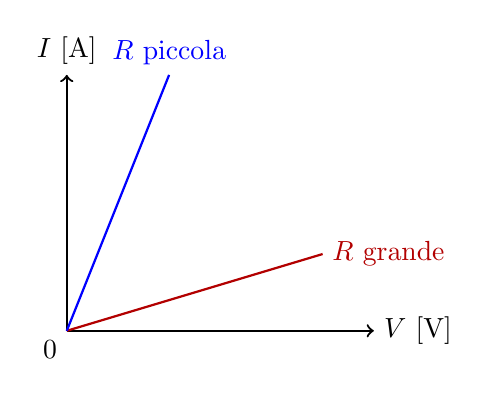
\begin{tikzpicture}[scale=0.65]
  % Assi
  \draw[->, thick] (0,0) -- (6,0) node[right] {\(V\) [V]};
  \draw[->, thick] (0,0) -- (0,5) node[above] {\(I\) [A]};

  % Retta per R grande (piatta)
  \draw[thick, red!70!black] (0,0) -- (5,1.5);
  \node[red!70!black, right] at (5,1.5) {\(R\) grande};

  % Retta per R piccola (ripida)
  \draw[thick, blue] (0,0) -- (2,5);
  \node[blue, above] at (2,5) {\(R\) piccola};

  % Etichetta origine
  \node[below left] at (0,0) {\(0\)};
\end{tikzpicture}
\end{minipage}

\begin{attenzione}
La legge di Ohm vale solo per i conduttori \textbf{ohmici}, cioè quelli per cui il rapporto \(\frac{V}{I}\) rimane costante al variare della tensione. Un filo metallico a temperatura costante è ohmico; altri componenti, come le lampadine a incandescenza, non seguono esattamente la legge di Ohm perché la loro resistenza cambia con la temperatura.
\end{attenzione}




\subsection{Il verso della corrente e il verso della tensione}

Consideriamo un resistore disposto orizzontalmente, percorso da una corrente \(I\) diretta verso destra. Ai suoi capi è applicata una tensione \(V\), rappresentata da una freccia diretta verso sinistra. A prima vista i due versi sembrano in contraddizione: perché mai la tensione “va” in senso opposto alla corrente?

\begin{figure}[htbp]
\centering
\begin{tikzpicture}[scale=1.2]
  % --- Resistore in orizzontale ---
% Vecchio: \resistoreANSI[0]{0}{0}{\(R\)}
  \resistoreANSI[label=$R_1$, label dx = 0, label dy = 0.6]{0}{0}
  % --- Frecce della corrente (verso destra) ---
  \draw[-, thick, black] (-1.5,0) -- (-1.2,0);
  \draw[->, thick, blue] (-1.2,0) -- (-1,0);
  \node[above, blue] at (-1.1,0.2) {\(I\)};

  \draw[->, thick, blue] (1,0) -- (1.2,0);
  \node[above, blue] at (1.15,0.2) {\(I\)};
  \draw[-, thick, black] (1.2,0) -- (1.5,0);

  % --- Freccia della tensione (verso sinistra) ---
  \draw[->, thick, red!70!black] (1.0,-0.7) -- (-1.0,-0.7);
  \node[below, red!70!black] at (0,-0.7) {\(V\)};

  % --- Etichette dei morsetti ---
  \node[above] at (-1.2,-0.6) {\(+\)};
  \node[above] at (1.2,-0.6) {\(-\)};

\end{tikzpicture}
\end{figure}

\paragraph{Perché i versi sono opposti.}
La discordanza è solo apparente e nasce dal modo in cui si definiscono \(I\) e \(V\).

\begin{itemize}[leftmargin=0.5cm]
  \item Il \textbf{verso della corrente} è convenzionale: si assume come flusso di \textbf{cariche positive}. Nei metalli si muovono gli elettroni (cariche negative) in verso opposto, ma la convenzione storica è quella delle cariche positive. Quindi la freccia blu verso destra indica il verso convenzionale di \(I\).
  \item Il \textbf{verso della tensione} è definito come differenza di potenziale \(V = V_A - V_B\), dove \(A\) è il punto verso cui punta la freccia. La freccia rossa va quindi dal potenziale \textbf{minore} al potenziale \textbf{maggiore}: indica il punto a potenziale più alto.
\end{itemize}

Nel disegno, il morsetto a sinistra è a potenziale maggiore (\(+\)) e quello a destra a potenziale minore (\(-\)). La corrente, spinta dal potenziale più alto a quello più basso, scorre da \textbf{sinistra verso destra}. La tensione, essendo definita come \(V_A - V_B\) con \(A\) il punto verso cui punta la freccia, punta invece da \textbf{destra verso sinistra}, cioè dal potenziale minore al maggiore. In questo modo i conti tornano: la corrente va verso destra (dal \(+\) al \(-\)), la tensione punta verso sinistra (dal \(-\) al \(+\)).


















\subsection{La seconda legge di Ohm}

La prima legge di Ohm lega tensione, corrente e resistenza, ma non spiega da che cosa dipenda la resistenza di un conduttore. La \textbf{seconda legge di Ohm} risponde a questa domanda: la resistenza di un conduttore dipende dal materiale di cui è fatto, dalla sua lunghezza e dalla sua sezione.

Riprendiamo il \textbf{provino cilindrico} dell'esperimento di Ohm: un filo di lunghezza \(l\) e sezione \(S\). La sua resistenza dipende da tre fattori:
\begin{itemize}[leftmargin=1cm]
  \item dal \textbf{materiale}: alcuni materiali conducono meglio di altri. Questa proprietà si chiama \textbf{resistività} e si indica con la lettera greca \(\rho\);
  \item dalla \textbf{lunghezza} del filo: più il filo è lungo, più le cariche devono attraversare materiale, e più la resistenza è alta. La resistenza è direttamente proporzionale alla lunghezza \(l\);
  \item dalla \textbf{sezione} del filo: più il filo è grosso, più spazio hanno le cariche per passare, e più la resistenza è bassa. La resistenza è inversamente proporzionale alla sezione \(S\).
\end{itemize}

La seconda legge di Ohm si esprime nella forma
\[
R = \rho \cdot \frac{l}{S},
\]
dove \(R\) è la resistenza [\(\Omega\)], \(\rho\) è la resistività del materiale [\(\Omega \cdot \text{mm}^2/\text{m}\)], \(l\) è la lunghezza [\(\text{m}\)] e \(S\) è la sezione trasversale [\(\text{mm}^2\)].

\subsection{I resistori e la simbologia}

Un componente progettato specificamente per avere una resistenza ben definita si chiama \textbf{resistore}. Nei circuiti si rappresenta in due modi:

\begin{figure}[htbp]
\centering

\begin{tikzpicture}[scale=1]
% Vecchio: \resistoreIEC{0}{0}{}
\resistoreIEC{0}{0}  \node[below] at (0,-1) {\textbf{Simbolo IEC}};
\resistoreANSI{4}{0}
  \node[below] at (4,-1) {\textbf{Simbolo ANSI}};
\end{tikzpicture}
\end{figure}

\begin{attenzione}
Il \textbf{simbolo IEC} (rettangolo) è quello più usato in Europa. Il \textbf{simbolo ANSI} (zigzag) è usato nel mondo anglosassone e in molti software di simulazione. In questa dispensa si utilizzerà prevalentemente il simbolo ANSI, che è quello più diffuso nei libri di testo in uso.
\end{attenzione}





\section{Il codice colori dei resistori}

I resistori sono spesso troppo piccoli per riportare stampato il loro valore. Per questo motivo si utilizza un codice normalizzato a bande colorate. Ogni banda corrisponde a una cifra, a un moltiplicatore, a una tolleranza oppure, nei resistori a 6 bande, a un coefficiente di temperatura.

Per leggere correttamente un resistore bisogna orientarlo nel verso giusto: si parte dal lato in cui le bande sono più vicine tra loro. La banda di tolleranza, invece, è generalmente separata dalle altre e si trova all'altra estremità. Se il resistore ha 6 bande, l'ultima banda è il coefficiente di temperatura.

\begin{concetto}
\textbf{Struttura generale del codice colori}

\begin{itemize}[leftmargin=1cm]
  \item \textbf{4 bande}: 1\textsuperscript{a} cifra, 2\textsuperscript{a} cifra, moltiplicatore, tolleranza;
  \item \textbf{5 bande}: 1\textsuperscript{a} cifra, 2\textsuperscript{a} cifra, 3\textsuperscript{a} cifra, moltiplicatore, tolleranza;
  \item \textbf{6 bande}: 1\textsuperscript{a} cifra, 2\textsuperscript{a} cifra, 3\textsuperscript{a} cifra, moltiplicatore, tolleranza, coefficiente di temperatura.
\end{itemize}
\end{concetto}

\begin{table}[htbp]
    \centering
    \small
    \begin{tabular}{c l c c c c}
    \hline
     & \textbf{Colore} & \textbf{Cifra} & \textbf{Moltiplicatore} & \textbf{Tolleranza} & \textbf{Coeff. temp.} \\
    \hline
    \colbox{black}   & Nero    & 0 & \(\times 10^0\) & --- & --- \\
    \colbox{brown}   & Marrone & 1 & \(\times 10^1\) & \(\pm 1\%\) & \(100\,\text{ppm}/^\circ\text{C}\) \\
    \colbox{red}     & Rosso   & 2 & \(\times 10^2\) & \(\pm 2\%\) & \(50\,\text{ppm}/^\circ\text{C}\) \\
    \colbox{orange}  & Arancione & 3 & \(\times 10^3\) & --- & \(15\,\text{ppm}/^\circ\text{C}\) \\
    \colbox{yellow}  & Giallo  & 4 & \(\times 10^4\) & --- & \(25\,\text{ppm}/^\circ\text{C}\) \\
    \colbox{green}   & Verde   & 5 & \(\times 10^5\) & \(\pm 0{,}5\%\) & --- \\
    \colbox{blue}    & Blu     & 6 & \(\times 10^6\) & \(\pm 0{,}25\%\) & \(10\,\text{ppm}/^\circ\text{C}\) \\
    \colbox{violet}  & Viola   & 7 & \(\times 10^7\) & \(\pm 0{,}1\%\) & \(5\,\text{ppm}/^\circ\text{C}\) \\
    \colbox{gray}    & Grigio  & 8 & \(\times 10^8\) & \(\pm 0{,}05\%\) & --- \\
    \colbox{white}   & Bianco  & 9 & \(\times 10^9\) & --- & --- \\
    \colbox{gold}    & Oro     & --- & \(\times 10^{-1}\) & \(\pm 5\%\) & --- \\
    \colbox{silver}  & Argento & --- & \(\times 10^{-2}\) & \(\pm 10\%\) & --- \\
    \hline
    \end{tabular}
    \end{table}

\subsection{Come calcolare il valore}

Per un resistore a \textbf{4 bande}, dette \(d_1\) e \(d_2\) le prime due cifre e \(m\) il moltiplicatore, si ha
\[
R = (10\,d_1 + d_2)\times 10^m\,[\Omega].
\]
La quarta banda indica la tolleranza.

Per un resistore a \textbf{5 bande} o a \textbf{6 bande}, dette \(d_1\), \(d_2\), \(d_3\) le prime tre cifre e \(m\) il moltiplicatore, si ha
\[
R = (100\,d_1 + 10\,d_2 + d_3)\times 10^m\,[\Omega].
\]
Nel resistore a 5 bande la quinta banda indica la tolleranza; nel resistore a 6 bande la quinta banda indica la tolleranza e la sesta il coefficiente di temperatura.

\begin{esempio}
\textbf{Resistore a 4 bande.} Le bande sono: giallo, viola, rosso, oro.

\begin{itemize}[leftmargin=1cm]
  \item giallo \(= 4\);
  \item viola \(= 7\);
  \item rosso \(= \times 10^2\);
  \item oro \(= \pm 5\%\).
\end{itemize}

Quindi
\[
R = 47 \times 10^2\,[\Omega] = 4700\,[\Omega] = 4{,}7\,[\text{k}\Omega],
\]
con tolleranza \(\pm 5\%\).
\end{esempio}

\begin{esempio}
\textbf{Resistore a 5 bande.} Le bande sono: rosso, viola, nero, marrone, marrone.

\begin{itemize}[leftmargin=1cm]
  \item rosso \(= 2\);
  \item viola \(= 7\);
  \item nero \(= 0\);
  \item marrone \(= \times 10^1\);
  \item marrone \(= \pm 1\%\).
\end{itemize}

Quindi
\[
R = 270 \times 10^1\,[\Omega] = 2700\,[\Omega] = 2{,}7\,[\text{k}\Omega] \pm 1\%,
\]
\end{esempio}

\begin{esempio}
\textbf{Resistore a 6 bande.} Le bande sono: rosso, viola, nero, marrone, marrone, rosso.

Il valore è ancora
\[
R = 2{,}7\,[\text{k}\Omega] \pm 1\%.
\]
La sesta banda, rossa, indica un coefficiente di temperatura di \(50\,\text{ppm}/^\circ\text{C}\).
\end{esempio}

\subsection{Le serie di valori normalizzati}

Con il termine \textbf{serie}, nel contesto dei resistori, si intendono le \textbf{serie E} di valori normalizzati. Non tutti i valori di resistenza esistono in commercio: i produttori realizzano solo alcuni valori standard, distribuiti in modo logaritmico all'interno di ogni decade.

Le serie più comuni sono:

\begin{itemize}[leftmargin=1cm]
  \item \textbf{E6}: 6 valori per decade, tolleranza tipica \(\pm 20\%\);
  \item \textbf{E12}: 12 valori per decade, tolleranza tipica \(\pm 10\%\);
  \item \textbf{E24}: 24 valori per decade, tolleranza tipica \(\pm 5\%\);
  \item \textbf{E48}: 48 valori per decade, tolleranza tipica \(\pm 2\%\);
  \item \textbf{E96}: 96 valori per decade, tolleranza tipica \(\pm 1\%\);
  \item \textbf{E192}: 192 valori per decade, tolleranza tipica \(\pm 0{,}5\%\).
\end{itemize}

Per esempio, nella serie E12 i valori principali sono:
\[
10,\ 12,\ 15,\ 18,\ 22,\ 27,\ 33,\ 39,\ 47,\ 56,\ 68,\ 82.
\]
Moltiplicando o dividendo questi valori per potenze di 10 si ottengono tutti gli altri valori della serie.

\begin{attenzione}
Non confondere le \textbf{serie E} con il collegamento in serie. Le serie E riguardano i valori commerciali normalizzati dei resistori; il collegamento in serie, invece, è un modo di collegare due o più componenti elettrici.
\end{attenzione}



\section{Esercizi}

\subsection{Domande di comprensione}

\begin{enumerate}[leftmargin=1cm]
  \item Perché si dice che la carica elettrica è una proprietà intrinseca della materia?
  \item Che cosa succede, dal punto di vista delle cariche, quando si strofina un palloncino sui capelli?
  \item Cosa indica il segno della forza di coulomb?
  \item Come si ricava l'unità di misura della costante \(k\) a partire dalla legge di Coulomb?
  \item Che cos'è il campo elettrico e perché si introduce una carica di prova per definirlo?
  \item In che direzione puntano le linee di campo di una carica positiva? E di una carica negativa? Qual è il significato fisico delle linee di campo?
  \item Che cos'è il lavoro elettrico? In quali casi è positivo e in quali è negativo?
  \item Che cos'è la tensione elettrica? In quale unità di misura si esprime?
  \item Definisci l'intensità di corrente.
  \item Che cos'è la resistenza elettrica e da quali fattori dipende?
\end{enumerate}

\subsection{Esercizi sulla forza di Coulomb}

\begin{esercizio}
\textbf{Esercizio svolto.} Due cariche puntiformi \(Q_1 = 2\,[\mu\text{C}]\) e \(Q_2 = 3\,[\mu\text{C}]\) sono poste a una distanza \(r = 10\,[\text{cm}]\). Calcolare il modulo della forza con cui interagiscono. Stabilire se è attrattiva o repulsiva.

\smallskip
\textbf{Soluzione.} Convertiamo le unità:
\[
Q_1 = 2 \times 10^{-6}\,[\text{C}], \quad Q_2 = 3 \times 10^{-6}\,[\text{C}], \quad r = 0{,}1\,[\text{m}].
\]
Applicando la legge di Coulomb:
\[
F = k\,\frac{Q_1\,Q_2}{r^2} = 8{,}99 \times 10^9 \cdot \frac{2\times 10^{-6} \cdot 3\times 10^{-6}}{(0{,}1)^2}.
\]
Svolgendo i calcoli:
\[
F = 8{,}99 \times 10^9 \cdot 6 \times 10^{-10} = 5{,}394\,[\text{N}].
\]
Poiché le due cariche sono concordi (entrambe positive), la forza è \textbf{repulsiva}.
\end{esercizio}

\textbf{Esercizi da svolgere.}
\begin{enumerate}[leftmargin=1cm]
  \item Due cariche \(Q_1 = 1\,[\mu\text{C}]\) e \(Q_2 = -2\,[\mu\text{C}]\) sono poste a distanza \(r = 5\,[\text{cm}]\). Calcolare il modulo della forza e stabilire se è attrattiva o repulsiva.
  \item Due cariche identiche \(Q\) sono poste a \(r = 20\,[\text{cm}]\) e si respingono con una forza di \(0{,}9\,[\text{N}]\). Calcolare il valore di \(Q\).
  \item Due cariche di \(4\,[\mu\text{C}]\) e \(6\,[\mu\text{C}]\) si trovano a distanza \(r\). Se la forza tra esse vale \(2{,}16\,[\text{N}]\), calcolare \(r\).
  \item Se la distanza tra due cariche triplica, come cambia il modulo della forza di Coulomb?
  \item Se una delle due cariche raddoppia e la distanza resta la stessa, come cambia il modulo della forza?
\end{enumerate}

\subsection{Esercizi sul campo elettrico}

\begin{esercizio}
\textbf{Esercizio svolto.} Una carica puntiforme \(Q = 5\,[\mu\text{C}]\) genera un campo elettrico nello spazio circostante. Calcolare il modulo del campo a una distanza \(r = 30\,[\text{cm}]\) dalla carica.

\smallskip
\textbf{Soluzione.} Convertiamo le unità: \(Q = 5 \times 10^{-6}\,[\text{C}]\), \(r = 0{,}3\,[\text{m}]\). Applicando la formula del campo di una carica puntiforme:
\[
E = k\,\frac{Q}{r^2} = 8{,}99 \times 10^9 \cdot \frac{5 \times 10^{-6}}{(0{,}3)^2}.
\]
Svolgendo i calcoli:
\[
E = 8{,}99 \times 10^9 \cdot \frac{5 \times 10^{-6}}{0{,}09} \approx 4{,}99 \times 10^5\,[\text{N/C}].
\]
Il campo è diretto verso l'esterno perché la carica è positiva.
\end{esercizio}

\textbf{Esercizi da svolgere.}
\begin{enumerate}[leftmargin=1cm]
  \item Una carica \(Q = 2\,[\mu\text{C}]\) genera un campo elettrico. Calcolare il valore del campo a distanza \(r = 10\,[\text{cm}]\).
  \item Una carica \(Q = -3\,[\mu\text{C}]\) genera un campo elettrico. Calcolare il valore del campo a distanza \(r = 15\,[\text{cm}]\) e indicare il verso delle linee di campo.
  \item In un punto dello spazio il campo elettrico vale \(E = 500\,[\text{N/C}]\). Una carica di prova \(q_0 = 2\,[\mu\text{C}]\) è posta in quel punto. Calcolare la forza che agisce su di essa.
  \item In un punto dello spazio agisce su una carica di prova \(q_0 = 5\,[\text{nC}]\) una forza di \(1\,[\mu\text{N}]\). Calcolare il modulo del campo elettrico in quel punto.
\end{enumerate}

\subsection{Esercizi su lavoro e tensione}

\begin{esercizio}
\textbf{Esercizio svolto.} In un campo elettrico uniforme di intensità \(E = 200\,[\text{N/C}]\), una carica \(Q = 3\,[\mu\text{C}]\) si sposta di \(s = 0{,}2\,[\text{m}]\) nella direzione del campo. Calcolare il lavoro elettrico compiuto e la tensione tra il punto iniziale e quello finale.

\smallskip
\textbf{Soluzione.} Convertiamo la carica in coulomb: \(Q = 3 \times 10^{-6}\,[\text{C}]\). Il lavoro elettrico è
\[
L_e = Q \cdot E \cdot s = 3 \times 10^{-6} \cdot 200 \cdot 0{,}2 = 1{,}2 \times 10^{-4}\,[\text{J}].
\]
La tensione è
\[
V = \frac{L_e}{Q} = E \cdot s = 200 \cdot 0{,}2 = 40\,[\text{V}].
\]
\end{esercizio}

\textbf{Esercizi da svolgere.}
\begin{enumerate}[leftmargin=1cm]
  \item Una carica \(Q = 1\,[\mu\text{C}]\) si sposta di \(0{,}5\,[\text{m}]\) in un campo di \(100\,[\text{N/C}]\). Calcolare il lavoro elettrico e la tensione.
  \item Tra due punti di un circuito esiste una tensione di \(12\,[\text{V}]\). Calcolare il lavoro necessario per spostare una carica di \(0{,}5\,[\text{C}]\) da un punto all'altro.
  \item Una carica di \(2\,[\text{C}]\) si sposta tra due punti tra i quali c'è una tensione di \(9\,[\text{V}]\). Calcolare il lavoro elettrico compiuto.
  \item Se tra due punti c'è una tensione di \(5\,[\text{V}]\) e viene compiuto un lavoro di \(0{,}25\,[\text{J}]\), quanta carica è stata spostata?
\end{enumerate}

\subsection{Esercizi su corrente e resistenza}

\begin{esercizio}
\textbf{Esercizio svolto.} In un conduttore circola una corrente \(I = 2\,[\text{A}]\) per un tempo \(\Delta t = 5\,[\text{s}]\). Calcolare la carica che ha attraversato una sezione del conduttore.

\smallskip
\textbf{Soluzione.} Applicando la formula inversa:
\[
\Delta Q = I \cdot \Delta t = 2 \cdot 5 = 10\,[\text{C}].
\]
\end{esercizio}

\begin{esercizio}
\textbf{Esercizio svolto.} Un resistore da \(R = 220\,[\Omega]\) è collegato a una batteria da \(V = 9\,[\text{V}]\). Calcolare la corrente che lo attraversa.

\smallskip
\textbf{Soluzione.} Applicando la legge di Ohm:
\[
I = \frac{V}{R} = \frac{9}{220} \approx 0{,}041\,[\text{A}] \approx 41\,[\text{mA}].
\]
\end{esercizio}

\textbf{Esercizi da svolgere.}
\begin{enumerate}[leftmargin=1cm]
  \item Una carica di \(50\,[\text{C}]\) attraversa un conduttore in \(10\,[\text{s}]\). Calcolare l'intensità di corrente.
  \item Una corrente di \(0{,}5\,[\text{A}]\) attraversa un conduttore per \(60\,[\text{s}]\). Calcolare la carica transitata.
  \item Un resistore da \(100\,[\Omega]\) è collegato a una tensione di \(5\,[\text{V}]\). Calcolare la corrente che lo attraversa.
  \item Un resistore è attraversato da una corrente di \(0{,}5\,[\text{A}]\) con una tensione ai capi di \(12\,[\text{V}]\). Calcolare il valore della resistenza.
  \item Calcolare la resistenza di un filo di rame lungo \(100\,[\text{m}]\) con una sezione di \(1\,[\text{mm}^2]\). La resistività del rame è \(\rho = 0{,}017\,[\Omega\cdot\text{mm}^2/\text{m}]\).
  \item Un filo di alluminio lungo \(50\,[\text{m}]\) ha sezione \(2\,[\text{mm}^2]\). Calcolare la sua resistenza, sapendo che \(\rho_{\text{Al}} = 0{,}028\,[\Omega\cdot\text{mm}^2/\text{m}]\).
\end{enumerate}

\subsection{Esercizi sul codice colori dei resistori}

\begin{esercizio}
\textbf{Esercizio svolto.} Un resistore ha le bande: marrone, nero, rosso, oro. Calcolare il valore e la tolleranza.

\smallskip
\textbf{Soluzione.} Le cifre sono \(1\) e \(0\), il moltiplicatore è \(\times 10^2\), la tolleranza è \(\pm 5\%\). Quindi
\[
R = 10 \times 10^2\,[\Omega] = 1000\,[\Omega] = 1\,[\text{k}\Omega] \pm 5\%.
\]
\end{esercizio}

\begin{esercizio}
\textbf{Esercizio svolto.} Un resistore a 5 bande ha le bande: verde, blu, nero, giallo, rosso. Calcolare il valore.

\smallskip
\textbf{Soluzione.} Le cifre sono \(5\), \(6\), \(0\); il moltiplicatore è \(\times 10^4\); la tolleranza è \(\pm 2\%\). Quindi
\[
R = 560 \times 10^4\,[\Omega] = 5\,600\,000\,[\Omega] = 5{,}6\,[\text{M}\Omega] \pm 2\%.
\]
\end{esercizio}

\textbf{Esercizi da svolgere.}

\begin{enumerate}[leftmargin=1cm]
  \item Un resistore a 4 bande ha i colori: rosso, rosso, marrone, argento. Calcolare il valore e la tolleranza.
  \item Un resistore a 4 bande ha i colori: giallo, viola, nero, oro. Calcolare il valore e la tolleranza.
  \item Un resistore a 5 bande ha i colori: arancione, arancione, nero, rosso, marrone. Calcolare il valore e la tolleranza.
  \item Un resistore a 6 bande ha i colori: marrone, nero, nero, rosso, oro, marrone. Calcolare valore, tolleranza e coefficiente di temperatura.
  \item Un resistore a 5 bande ha i colori: marrone, nero, nero, marrone, marrone. Calcolare il valore.
  \item Quante cifre significative si leggono in un resistore a 4 bande? E in uno a 5 bande? E in uno a 6 bande?
  \item Perché la banda di tolleranza è generalmente separata dalle altre?
  \item Che cosa indica la sesta banda in un resistore a 6 bande?
  \item Che cosa sono le serie E? Perché esistono?
  \item Un resistore da \(4{,}7\,[\text{k}\Omega] \pm 5\%\) viene rappresentato con 4 bande. Quali colori possono comparire?
\end{enumerate}

\chapter{Circuiti elettrici e leggi di Kirchhoff}

\begin{concetto}
Questo capitolo introduce i concetti fondamentali della teoria dei circuiti: che cos'è un circuito elettrico, che cosa sono un nodo e una maglia, e come si applicano le due leggi di Kirchhoff per analizzare circuiti semplici. Le leggi di Kirchhoff sono gli strumenti di base per risolvere qualsiasi circuito, dal più semplice al più complesso, e costituiscono il ponte tra i concetti di tensione e corrente introdotti nel capitolo precedente e la risoluzione concreta dei problemi circuitali.
\end{concetto}

\section{Che cos'è un circuito elettrico}

Un \textbf{circuito elettrico} è un insieme di componenti elettrici collegati tra loro in modo da formare un \textbf{percorso chiuso} attraverso il quale può fluire la corrente elettrica. Il percorso chiuso è la condizione essenziale: se il percorso non è chiuso, la corrente non può circolare.

I componenti che si incontrano in un circuito si possono raggruppare in tre categorie fondamentali:

\begin{concetto}
\textbf{Componenti fondamentali di un circuito}
\begin{itemize}[leftmargin=1cm]
  \item i \textbf{generatori}, che mantengono una differenza di potenziale tra i loro terminali e forniscono energia al circuito (pile, batterie, alimentatori);
  \item i \textbf{conduttori}, cioè i fili che collegano tra loro i componenti e permettono il passaggio della corrente;
  \item gli \textbf{utilizzatori}, che assorbono energia elettrica e la trasformano in altre forme di energia (lampadine, resistori, motori).
\end{itemize}
\end{concetto}

Un circuito si dice \textbf{aperto} quando il percorso è interrotto in almeno un punto: in questo caso la corrente non circola. Si dice \textbf{chiuso} quando il percorso è completo: la corrente può circolare. Un interruttore è un dispositivo che permette di aprire o chiudere volontariamente un circuito.

\begin{esempio}
\textbf{La torcia.} Una torcia è un circuito semplicissimo: una pila , due fili, una lampadina e un interruttore. Quando l'interruttore è chiuso, il percorso è completo, la corrente circola e la lampadina si accende. Quando l'interruttore è aperto, il percorso è interrotto e la lampadina si spegne.
\end{esempio}

\begin{attenzione}
In un circuito reale i fili hanno una resistenza piccolissima ma non nulla. Nei circuiti ideali, che sono quelli che si studiano in questa sede, i fili si considerano conduttori perfetti, cioè con resistenza nulla.
\end{attenzione}

\subsection{Il nodo}

In un circuito possono incontrarsi più conduttori nello stesso punto. Questo punto prende il nome di \textbf{nodo}.

\begin{concetto}
Un \textbf{nodo} è un punto del circuito in cui convergono \textbf{tre o più} conduttori. Due soli conduttori che si incontrano non formano un nodo, perché non c'è alcuna suddivisione della corrente: il punto è semplicemente un punto di collegamento tra due componenti in serie.
\end{concetto}

\begin{figure}[htbp]
\centering
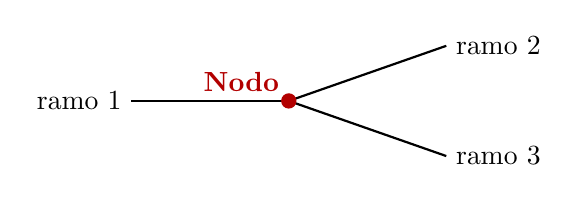
\begin{tikzpicture}[scale=1]
  % Rami che convergono nel nodo
  \draw[thick] (-2,0) -- (0,0);
  \draw[thick] (0,0) -- (2,0.7);
  \draw[thick] (0,0) -- (2,-0.7);
  % Nodo
  \filldraw[red!70!black] (0,0) circle (0.09);
  \node[above left, red!70!black] at (0,0) {\textbf{Nodo}};
  % Etichette dei rami
  \node[left] at (-2,0) {ramo 1};
  \node[right] at (2,0.7) {ramo 2};
  \node[right] at (2,-0.7) {ramo 3};
\end{tikzpicture}
\end{figure}

\begin{esempio}
In un circuito con una pila e due lampadine collegate in parallelo, il polo positivo della pila è collegato a un punto in cui il filo si dirama verso le due lampadine: quel punto è un nodo. Lo stesso vale per il polo negativo.
\end{esempio}

\subsection{La maglia}

Un altro concetto fondamentale è quello di maglia.

\begin{concetto}
Una \textbf{maglia} è un qualsiasi percorso chiuso non intrecciato che parte da un nodo e ritorna allo stesso nodo senza passare due volte per lo stesso ramo. In altre parole, è un anello chiuso all'interno del circuito.
\end{concetto}

Una maglia può contenere al suo interno altri percorsi chiusi oppure no. Quando non ne contiene, si parla di \textbf{maglia elementare}.

\begin{concetto}
Una \textbf{maglia elementare} (o maglia semplice) è una maglia che non contiene al suo interno altre maglie. In pratica, è il più piccolo anello chiuso che si può individuare in un circuito.
\end{concetto}

\begin{attenzione}
Saper distinguere tra maglie elementari e non elementari è importante perché, applicando la legge delle maglie, si scelgono di norma le maglie elementari. Le maglie non elementari danno equazioni che sono combinazione lineare di quelle elementari e non aggiungono informazione.
\end{attenzione}




\section{La legge di Kirchhoff alle Tensioni (legge delle maglie)}

\begin{concetto}
\textbf{LKT (legge delle maglie).} La somma algebrica delle tensioni lungo una maglia è nulla:
\[
\sum_k V_k = 0.
\]
Equivalentemente, la somma delle forze elettromotrici presenti nella maglia è uguale alla somma delle cadute di tensione sui resistori:
\[
\sum \mathcal{E} = \sum R\,I.
\]
\end{concetto}

Questa legge esprime il fatto che, percorrendo un percorso chiuso, si ritorna al punto di partenza con lo stesso potenziale: la somma dei guadagni di tensione deve uguagliare la somma delle perdite.

\subsection{La convenzione dei segni}

Per applicare correttamente la seconda legge di Kirchhoff bisogna fissare una \textbf{convenzione dei segni} e seguirla con coerenza. La procedura è la seguente:

\begin{enumerate}[leftmargin=1cm]
  \item si sceglie arbitrariamente un \textbf{verso di percorrenza} della maglia (orario o antiorario);
  \item per ogni \textbf{generatore} incontrato lungo il percorso, si attribuisce segno \(+\) se si passa dal polo negativo al polo positivo (guadagno di tensione), segno \(-\) se si passa dal polo positivo al polo negativo;
  \item per ogni \textbf{resistore} percorso da una corrente \(I\), si attribuisce segno \(-\) alla caduta \(RI\).
\end{enumerate}

In forma compatta, scrivendo \(\sum V_k = 0\) con questa convenzione, si ottiene direttamente l'equazione risolutiva.

\begin{attenzione}
Il verso di percorrenza scelto è arbitrario: cambiandolo si ottiene un'equazione equivalente, moltiplicata per \(-1\). Il risultato finale non cambia. La cosa importante è non cambiare convenzione a metà calcolo.
\end{attenzione}

\subsection{Esempio di applicazione}

\begin{esempio}
\textbf{Circuito con un solo anello.} Si consideri un circuito formato da una pila con forza elettromotrice \(\mathcal{E} = 12\,[\text{V}]\) e due resistori in serie, \(R_1 = 4\,[\Omega]\) e \(R_2 = 2\,[\Omega]\). Calcolare la corrente che circola nel circuito.

\smallskip
\textbf{Soluzione.} Il circuito ha una sola maglia. Scegliamo come verso di percorrenza quello orario. Percorrendo la maglia:

\begin{itemize}[leftmargin=1cm]
  \item attraverso la pila si passa dal polo negativo al polo positivo: guadagno \(+\mathcal{E}\);
  \item attraverso \(R_1\) la corrente ha lo stesso verso del percorso: caduta \(-R_1 I\);
  \item attraverso \(R_2\) la corrente ha lo stesso verso del percorso: caduta \(-R_2 I\).
\end{itemize}

La seconda legge di Kirchhoff fornisce
\[
\mathcal{E} - R_1 I - R_2 I = 0.
\]
Da cui
\[
I = \frac{\mathcal{E}}{R_1 + R_2} = \frac{12}{4 + 2} = 2\,[\text{A}].
\]
\end{esempio}

\subsection{Esempio con più generatori}

\begin{esempio}
\textbf{Circuito con due generatori.} Si consideri una maglia singola formata da:
\begin{itemize}[leftmargin=1cm]
  \item due generatori \(\mathcal{E}_1 = 12\,[\text{V}]\) e \(\mathcal{E}_2 = 6\,[\text{V}]\);
  \item due resistori, \(R_1 = 3\,[\Omega]\) e \(R_2 = 1\,[\Omega]\).
\end{itemize}
I due generatori sono disposti in modo che \(\mathcal{E}_1\) favorisca la corrente nel verso orario, mentre \(\mathcal{E}_2\) si opponga. Calcolare la corrente \(I\) che circola nella maglia.

\smallskip
\textbf{Soluzione.} Scegliamo come verso di percorrenza quello orario. Rappresentiamo la maglia e indichiamo con frecce le tensioni incontrate lungo il percorso.



\begin{center}
\begin{tikzpicture}[scale=1]
  % --- Maglia rettangolare con interruzioni per i resistori ---
  % Lato sinistro (generatore 1): linea continua
  \draw[thick] (0,0) -- (0,3);
  % Lato destro (generatore 2): linea continua
  \draw[thick] (6,0) -- (6,3);
  % Lato superiore: interrotto al centro per R1
  \draw[thick] (0,3) -- (2,3);
  \draw[thick] (4,3) -- (6,3);
  % Lato inferiore: interrotto al centro per R2
  \draw[thick] (0,0) -- (2,0);
  \draw[thick] (4,0) -- (6,0);

  % --- Generatore 1 (lato sinistro, + in alto) ---
  % Sostituisci: \generatore[0]{0}{1.5}{}
\generatore[rot=0]{0}{1.5}
\generatore[rot=0]{6}{1.5}

  % --- Resistore R1 (lato superiore) ---
  % Sostituisci: \resistoreANSI[0]{3}{3}{}
\resistoreANSI[rot=0, label = $R_1$, label dy = -0.5]{3}{3}
\resistoreANSI[rot=0, label = $R_2$, label dy = 0.5]{3}{0}

  % --- Frecce per le tensioni (all'esterno della maglia) ---

  % Generatore 1: dal basso verso l'alto (guadagno +E1)
  \draw[->, thick, rossoscuro] (-0.6,0.5) -- (-0.6,2.5);
  \node[left, rossoscuro] at (-0.6,1.5) {\(+\mathcal{E}_1\)};

  % Generatore 2: dal basso verso l'alto (guadagno +E2)
  \draw[->, thick, rossoscuro] (6.6,0.5) -- (6.6,2.5);
  \node[right, rossoscuro] at (6.6,1.5) {\(+\mathcal{E}_2\)};

  % Resistore R1: verso orario (da sinistra a destra)
  \draw[->, thick, blue] (4,3.6) -- (2,3.6);
  \node[above, blue] at (3,3.6) {\(V_1\)};

  % Resistore R2: verso orario (da destra a sinistra)
  \draw[->, thick, blue] (2,-0.6) -- (4,-0.6);
  \node[below, blue] at (3,-0.6) {\(V_2\)};

  % Verso di percorrenza orario (freccia curva al centro)
  \draw[->, thick, green!60!black] (1.8,0.9) arc (170:10:1.2);
  \node[green!60!black] at (3,1.2) {verso orario};
\end{tikzpicture}
\end{center}







Percorrendo la maglia in verso orario:
\begin{itemize}[leftmargin=1cm]
  \item attraverso \(\mathcal{E}_1\) si passa dal polo negativo al polo positivo: guadagno \(+\mathcal{E}_1\);
  \item attraverso \(R_1\) e \(R_2\): caduta \(V_1 = -R_1 I\) e \(V_2 = -R_2 I\);
  \item attraverso \(\mathcal{E}_2\) si passa dal polo positivo al polo negativo: guadagno \(-\mathcal{E}_2\);
\end{itemize}

La legge di Kirchhoff alle Tensioni (LKT) fornisce:
\[
\mathcal{E}_1 - V_1 - \mathcal{E}_2 - V_2 = 0 \qquad\Longrightarrow\qquad
\mathcal{E}_1 - R_1 I - \mathcal{E}_2 - R_2 I = 0.
\]
Sostituendo i valori:
\[
12 - 3I - 6 - 1I = 0
\quad\Rightarrow\quad
6 - 4I = 0
\quad\Rightarrow\quad
I = \frac{6}{4} = 1.5\,[\text{A}].
\]
La corrente positiva indica che il verso effettivo è quello orario, cioè quello scelto.
\end{esempio}

\begin{curiosita}
Le leggi di Kirchhoff valgono per qualsiasi circuito, indipendentemente dal numero di componenti. Anche i circuiti integrati più complessi, con miliardi di transistori, vengono analizzati con gli stessi due principi. La potenza del metodo sta nella sua semplicità: due leggi, applicate con coerenza, bastano per risolvere qualsiasi rete lineare.
\end{curiosita}





\section{La legge di Kirchhoff alle Correnti (legge dei nodi)}
\begin{concetto}
\textbf{LKC (legge dei nodi).} In un nodo, la somma delle correnti che entrano è uguale alla somma delle correnti che escono:
\[
\sum I_{\text{entranti}} = \sum I_{\text{uscenti}}.
\]
Equivalentemente, attribuendo segno positivo alle correnti entranti e negativo a quelle uscenti (o viceversa), la somma algebrica di tutte le correnti che confluiscono in un nodo è nulla:
\[
\sum_k I_k = 0.
\]
\end{concetto}

Questa legge esprime un principio di conservazione: la carica elettrica non può accumularsi in un nodo né sparire, quindi tanta carica entra quanta esce nell'unità di tempo.

\begin{esempio}
\textbf{Nodo con tre rami.} In un nodo convergono tre conduttori. Nel primo entra una corrente \(I_1 = 3\,[\text{A}]\), nel secondo entra una corrente \(I_2 = 1\,[\text{A}]\). Quanta corrente esce dal terzo ramo?

\smallskip
\textbf{Soluzione.} Applichiamo la legge dei nodi:
\[
I_1 + I_2 = I_3 \quad \Longrightarrow \quad I_3 = 3 + 1 = 4\,[\text{A}].
\]
Dal terzo ramo escono \(4\,[\text{A}]\).
\end{esempio}

\begin{esempio}
\textbf{Nodo con quattro rami.} In un nodo entrano \(I_1 = 5\,[\text{A}]\) e \(I_2 = 2\,[\text{A}]\), mentre escono \(I_3 = 3\,[\text{A}]\) e \(I_4\) incognita. Determinare \(I_4\).

\smallskip
\textbf{Soluzione.}
\[
I_1 + I_2 = I_3 + I_4 \quad \Longrightarrow \quad 5 + 2 = 3 + I_4 \quad \Longrightarrow \quad I_4 = 4\,[\text{A}].
\]
\end{esempio}


\section{La massa}

\begin{concetto}
La \textbf{massa} (in inglese \textit{ground}, spesso indicata con il simbolo \(\bot\) o GND) è un \textbf{punto di riferimento} del circuito al quale si attribuisce per convenzione il potenziale elettrico \(V = 0\,[\text{V}]\). Tutti gli altri potenziali del circuito vengono misurati rispetto a questo punto.
\end{concetto}

\subsection{Perché serve un riferimento}

Una tensione non è mai un valore assoluto: è sempre una \textbf{differenza di potenziale tra due punti}. Dire ``in questo punto c'è una tensione di \(5\,[\text{V}]\)'' non ha senso se non si specifica \emph{rispetto a che cosa}.

Per capirlo, si può pensare all'altezza. Se si dice ``sono alto \(10\,[\text{m}]\)'', la frase è ambigua: \(10\,[\text{m}]\) rispetto a cosa? Se ci si trova al secondo piano di un palazzo, l'altezza rispetto al pavimento del piano è circa \(1{,}7\,[\text{m}]\), mentre l'altezza rispetto al livello del mare è molto maggiore. L'``altezza'' cambia a seconda del \textbf{riferimento} scelto. Eppure la posizione fisica è sempre la stessa: quello che cambia è solo il numero usato per descriverla.

Lo stesso vale per il potenziale elettrico. In un circuito, il potenziale di un nodo non ha un valore assoluto: ha senso solo se confrontato con un altro nodo. Per evitare di dover specificare ogni volta ``rispetto a questo nodo'', si sceglie un nodo di riferimento e lo si chiama \textbf{massa}. A quel nodo si assegna \(V = 0\,[\text{V}]\), e tutti gli altri potenziali si misurano rispetto a lui.

\begin{esempio}
\textbf{L'analogia del palazzo.}
\begin{itemize}[leftmargin=1cm]
  \item Il \textbf{pavimento del piano} è come la massa: è il livello rispetto al quale si misurano tutte le altezze dentro quell'appartamento.
  \item L'altezza di una persona (\(1{,}7\,[\text{m}]\)) è come la tensione di un nodo rispetto alla massa.
  \item Cambiando appartamento e prendendo come riferimento un altro pavimento, i numeri cambiano, ma la posizione fisica no.
  \item La differenza di altezza tra due persone (per esempio \(20\,[\text{cm}]\)) è come una \textbf{differenza di potenziale}: è quella che conta davvero, e non dipende dal riferimento scelto.
\end{itemize}
\end{esempio}

\subsection{Che cosa cambia e che cosa no}

\begin{itemize}[leftmargin=1cm]
  \item \textbf{Cambia} il valore numerico dei potenziali: spostando la massa in un altro punto, tutti i potenziali cambiano dello stesso valore.
  \item \textbf{Non cambiano} le \textbf{differenze di potenziale} tra i nodi, cioè le tensioni che compaiono nelle leggi di Kirchhoff e nella legge di Ohm.
  \item \textbf{Non cambiano} le correnti, perché esse dipendono solo dalle differenze di potenziale.
\end{itemize}

Per questo la scelta della massa è \textbf{arbitraria}: il funzionamento del circuito non dipende da dove viene messa. È solo una convenzione comoda, che permette di parlare di ``potenziale di un nodo'' senza specificare ogni volta rispetto a che cosa.

\begin{attenzione}
La massa \textbf{non è} un componente che ``assorbe'' corrente o che ``scarica'' la corrente a terra. È solo un'\textbf{etichetta} che indica: ``questo nodo è il riferimento, il suo potenziale vale \(0\,[\text{V}]\)''. Nei circuiti reali la massa è spesso collegata allo chassis metallico del dispositivo o alla terra vera e propria (impianto di terra), ma concettualmente è solo un punto scelto come riferimento.
\end{attenzione}

\subsection{Il simbolo}

Nei circuiti la massa si rappresenta con un simbolo formato da tre linee orizzontali di lunghezza decrescente, oppure con un triangolino. Il filo che arriva al simbolo indica il nodo scelto come riferimento.

\begin{center}
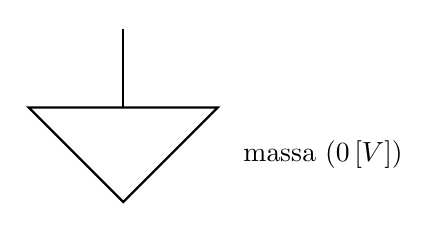
\begin{tikzpicture}[scale=2]
  % Filo
  \draw[thick] (0,0) -- (0,-0.5);
  % Triangolo
  \draw[thick] (-0.6,-0.5) -- (0.6,-0.5) -- (0,-1.1) -- cycle;
  % Etichetta
  \node[right] at (0.7,-0.8) {massa (\(0\,[\text{V}]\))};
\end{tikzpicture}
\end{center}


\begin{curiosita}
Nella maggior parte dei circuiti elettronici la massa è il nodo con più connessioni: è il ``filo comune'' a cui fanno riferimento tutti i segnali. Nei telefoni, nei computer e in quasi tutti i dispositivi elettronici, la massa è il punto rispetto al quale si misura ogni tensione. Senza un riferimento comune, parlare di ``\(3{,}3\,[\text{V}]\)'' o ``\(5\,[\text{V}]\)'' non avrebbe alcun significato.
\end{curiosita}
















\section{Partitore di tensione}

\begin{concetto}
Il \textbf{partitore di tensione} è un circuito formato da due o più resistori in serie. Esso permette di ottenere, ai capi di un resistore, una frazione della tensione totale applicata. È una conseguenza della legge di Ohm e della legge di Kirchhoff alle tensioni.
\end{concetto}

\subsection{Circuito con due resistori in serie}

Si consideri una serie di due resistori \(R_1\) e \(R_2\) alimentata da una tensione \(V_{\text{in}}\). La tensione di uscita \(V_{\text{out}}\) è prelevata ai capi di \(R_2\). Il terminale negativo del generatore è collegato alla \textbf{massa}, cioè al nodo di riferimento a cui si attribuisce \(V = 0\,[\text{V}]\).

\begin{center}
\begin{tikzpicture}[scale=1]
  % Filo sinistro dal basso al generatore
  \draw[thick] (0,0) -- (0,1.2);
  % Generatore
  \generatore{0}{2}{}
  \draw node[left] at (-0.5,2) {\(V_{\text{in}}\)};
  % Filo dal generatore al lato superiore
  \draw[thick] (0,2.8) -- (0,4);
  % Filo superiore fino al resistore R1
  \draw[thick] (0,4) -- (1,4);
  % Resistore R1
  \resistoreANSI[label = $R_1$, label dy = -0.5]{2}{4}
  \resistoreANSI[rot = 90, label = $R_2$, label dx = -0.6, label dy = 0]{4}{2}
  
  \draw[thick] (3,4) -- (4,4);
  \draw[thick] (4,4) -- (4,3);
  \draw[thick] (4,1) -- (4,0);
  \draw[thick] (4,0) -- (0,0);

  \massa{4}{0}

  \draw[thick] (4,0) -- (4.5,0);
  \draw[thick] (4,4) -- (4.5,4);
  \draw[thick] (4.6,4) circle (0.1);
  \draw[thick] (4.6,0) circle (0.1);
  % Etichetta V_out
  \draw[->, thick, red] (4.7,0.5) -- (4.7,3.5) node[midway,right] {\(V_{\text{out}}\)};
\end{tikzpicture}
\end{center}

\paragraph{Dimostrazione.}
Poiché \(R_1\) e \(R_2\) sono in serie, sono percorsi dalla stessa corrente \(I\). Applicando la legge di Kirchhoff alle tensioni all'unica maglia:

\[
V_{\text{in}} = V_{R_1} + V_{R_2}.
\]

Per la legge di Ohm:

\[
V_{R_1} = R_1 I, \qquad V_{R_2} = R_2 I.
\]

Sostituendo:

\[
V_{\text{in}} = R_1 I + R_2 I = (R_1 + R_2) I.
\]

Da cui la corrente:

\[
I = \frac{V_{\text{in}}}{R_1 + R_2}.
\]

La tensione ai capi di \(R_2\) è:

\[
V_{\text{out}} = V_{R_2} = R_2 I = R_2 \frac{V_{\text{in}}}{R_1 + R_2}.
\]

Quindi la formula del partitore di tensione è:

\[
\boxed{
V_{\text{out}} = V_{\text{in}} \frac{R_2}{R_1 + R_2}
}
\]

Analogamente, la tensione ai capi di \(R_1\) sarebbe \(V_{R_1} = V_{\text{in}} \frac{R_1}{R_1 + R_2}\).

\paragraph{Proprietà.}
Il resistore più grande ha ai suoi capi la tensione maggiore.
\subsection{Esempio numerico}

Un partitore di tensione ha \(V_{\text{in}} = 12\,[\text{V}]\), \(R_1 = 4\,[\Omega]\), \(R_2 = 2\,[\Omega]\). Calcolare \(V_{\text{out}}\) ai capi di \(R_2\).

\[
V_{\text{out}} = 12 \cdot \frac{2}{4+2} = 12 \cdot \frac{2}{6} = 4\,[\text{V}].
\]

\section{Partitore di corrente}

\begin{concetto}
Il \textbf{partitore di corrente} è un circuito formato da due o più resistori in parallelo. Esso permette di dividere una corrente totale in più rami. La corrente in ciascun ramo è inversamente proporzionale alla resistenza del ramo stesso.
\end{concetto}

\subsection{Circuito con due resistori in parallelo}

Si considerino due resistori \(R_1\) e \(R_2\) collegati in parallelo, alimentati da una corrente totale \(I_{\text{tot}}\). La corrente si divide nei due rami in \(I_1\) e \(I_2\). Il nodo inferiore destro è collegato alla \textbf{massa}, cioè al riferimento a cui si attribuisce \(V = 0\,[\text{V}]\).

\begin{center}
\begin{tikzpicture}[scale=1]
  % Rail superiore
  \draw[thick] (0,4) -- (4,4);
  % Rail inferiore
  \draw[thick] (0,0) -- (4,0);

  % Ramo sinistro con generatore
  \draw[thick] (0,0) -- (0,1.2);
  \generatore{0}{2}
  \draw[thick] (0,2.8) -- (0,4);

  % Ramo con R1 (verticale, x=2)
  \draw[thick] (2,4) -- (2,3);
  \resistoreANSI[rot=90, label=$R_1$, label dx = 0.5, label dy = 0]{2}{2}
  \draw[thick] (2,1) -- (2,0);

  % Ramo con R2 (verticale, x=4)
  \draw[thick] (4,4) -- (4,3);
  \resistoreANSI[rot=90, label=$R_2$, label dx = 0.5, label dy = 0]{4}{2}
  \draw[thick] (4,1) -- (4,0);

  % Corrente totale sul rail superiore
  \draw[->, thick, rossoscuro] (0.5,4.25) -- (1.5,4.25) node[midway,above] {\(I_{\text{tot}}\)};

  % Correnti nei rami (verso il basso)
  \draw[->, thick, bluscuro] (2,3.7) -- (2,3.1) node[midway,right] {\(I_1\)};
  \draw[->, thick, bluscuro] (4,3.7) -- (4,3.1) node[midway,right] {\(I_2\)};

  % Nodi (punti di biforcazione)
  \filldraw (2,4) circle (0.05);
  \filldraw (4,4) circle (0.05);
  \filldraw (2,0) circle (0.05);
  \filldraw (4,0) circle (0.05);

  % Massa
  \massa{3}{0}
\end{tikzpicture}
\end{center}

\paragraph{Dimostrazione.}
Poiché \(R_1\) e \(R_2\) sono in parallelo, ai loro capi c'è la stessa tensione \(V\), misurata rispetto alla massa. Per la legge di Kirchhoff alle correnti applicata al nodo di ingresso:

\[
I_{\text{tot}} = I_1 + I_2.
\]

Per la legge di Ohm:

\[
I_1 = \frac{V}{R_1}, \qquad I_2 = \frac{V}{R_2}.
\]

Sostituendo:

\[
I_{\text{tot}} = \frac{V}{R_1} + \frac{V}{R_2} = V \left( \frac{1}{R_1} + \frac{1}{R_2} \right) = V\, \frac{R_1 + R_2}{R_1 R_2}.
\]

Quindi:

\[
I_{\text{tot}} = V \frac{R_1 + R_2}{R_1 R_2} \quad\Longrightarrow\quad V = I_{\text{tot}} \frac{R_1 R_2}{R_1 + R_2}.
\]

Ora si calcolano le correnti nei due rami:

\[
I_1 = \frac{V}{R_1} = \frac{1}{R_1} I_{\text{tot}} \frac{R_1 R_2}{R_1 + R_2} = I_{\text{tot}} \frac{R_2}{R_1 + R_2}.
\]

\[
I_2 = \frac{V}{R_2} = \frac{1}{R_2} I_{\text{tot}} \frac{R_1 R_2}{R_1 + R_2} = I_{\text{tot}} \frac{R_1}{R_1 + R_2}.
\]

Pertanto le formule del partitore di corrente sono:

\[
\boxed{
I_1 = I_{\text{tot}} \frac{R_2}{R_1 + R_2}
}
\qquad
\boxed{
I_2 = I_{\text{tot}} \frac{R_1}{R_1 + R_2}
}
\]

\paragraph{Proprietà.}
\begin{itemize}[leftmargin=1cm]
  \item La corrente si ripartisce in proporzione inversa alle resistenze: \(\frac{I_1}{I_2} = \frac{R_2}{R_1}\).
  \item Il ramo con resistenza maggiore è percorso da corrente minore.
\end{itemize}

\subsection{Esempio numerico}

Un partitore di corrente ha \(I_{\text{tot}} = 6\,[\text{A}]\), \(R_1 = 2\,[\Omega]\), \(R_2 = 4\,[\Omega]\). Calcolare \(I_1\) e \(I_2\).

\[
I_1 = 6 \cdot \frac{4}{2+4} = 6 \cdot \frac{4}{6} = 4\,[\text{A}],
\]

\[
I_2 = 6 \cdot \frac{2}{2+4} = 6 \cdot \frac{2}{6} = 2\,[\text{A}].
\]

Verifica: \(I_1 + I_2 = 4 + 2 = 6\,[\text{A}] = I_{\text{tot}}\).



\section{Esercizi}

\subsection{Domande di comprensione}

\begin{enumerate}[leftmargin=1cm]
  \item Che cos'è un circuito elettrico e perché deve essere chiuso perché la corrente circoli?
  \item Quali sono i tre tipi di componenti fondamentali di un circuito? Fai un esempio per ciascuno.
  \item Che cos'è un nodo? Perché due soli conduttori che si incontrano non formano un nodo?
  \item Che cos'è una maglia? Che differenza c'è tra maglia e maglia elementare?
  \item Enuncia la prima legge di Kirchhoff e spiega il significato fisico.
  \item Enuncia la seconda legge di Kirchhoff e spiega il significato fisico.
  \item Qual è la convenzione dei segni da usare nella legge delle maglie? Perché è importante non cambiarla a metà calcolo?
  \item Perché, applicando la legge delle maglie, conviene scegliere le maglie elementari?
  \item Quante equazioni indipendenti si possono scrivere ai nodi di un circuito con \(n\) nodi? E quante alle maglie?
\end{enumerate}

\subsection{Esercizi sui nodi}

\begin{esercizio}
\textbf{Esercizio svolto.} In un nodo convergono quattro conduttori. Entrano \(I_1 = 4\,[\text{A}]\) e \(I_2 = 3\,[\text{A}]\); esce \(I_3 = 5\,[\text{A}]\). Calcolare la corrente \(I_4\) nel quarto ramo.

\smallskip
\textbf{Soluzione.} Applichiamo la prima legge di Kirchhoff:
\[
I_1 + I_2 = I_3 + I_4.
\]
Sostituendo i valori:
\[
4 + 3 = 5 + I_4 \quad \Longrightarrow \quad I_4 = 2\,[\text{A}].
\]
La corrente \(I_4\) esce dal nodo.
\end{esercizio}

\textbf{Esercizi da svolgere.}

\begin{enumerate}[leftmargin=1cm]
  \item In un nodo entrano \(I_1 = 6\,[\text{A}]\) e \(I_2 = 2\,[\text{A}]\), ed esce \(I_3 = 5\,[\text{A}]\). Calcolare la corrente nel quarto ramo e stabilirne il verso.
  \item In un nodo convergono cinque rami: entrano \(I_1 = 3\,[\text{A}]\), \(I_2 = 4\,[\text{A}]\), \(I_3 = 1\,[\text{A}]\); esce \(I_4 = 2\,[\text{A}]\). Calcolare \(I_5\).
  \item In un nodo entrano tre correnti: \(I_1 = 1{,}5\,[\text{A}]\), \(I_2 = 2{,}5\,[\text{A}]\), \(I_3 = 3\,[\text{A}]\). Escono due correnti: \(I_4 = 4\,[\text{A}]\) e \(I_5\). Calcolare \(I_5\).
  \item In un nodo la somma delle correnti entranti è \(10\,[\text{A}]\). Se le correnti uscenti sono tre e valgono \(I_1 = 2\,[\text{A}]\), \(I_2 = 3\,[\text{A}]\), calcolare \(I_3\).
  \item In un nodo entrano \(I_1 = 2\,[\text{A}]\) e \(I_2 = 3\,[\text{A}]\), mentre esce \(I_3 = 7\,[\text{A}]\). È possibile? Giustifica la risposta.
\end{enumerate}

\subsection{Esercizi sulle maglie}

\begin{esercizio}
\textbf{Esercizio svolto.} In una maglia sono presenti una pila con \(\mathcal{E} = 9\,[\text{V}]\) e tre resistori in serie, \(R_1 = 1\,[\Omega]\), \(R_2 = 2\,[\Omega]\), \(R_3 = 3\,[\Omega]\). Calcolare la corrente che circola.

\smallskip
\textbf{Soluzione.} Applichiamo la seconda legge di Kirchhoff scegliendo come verso di percorrenza quello orario:
\[
\mathcal{E} - R_1 I - R_2 I - R_3 I = 0.
\]
Da cui
\[
I = \frac{\mathcal{E}}{R_1 + R_2 + R_3} = \frac{9}{1 + 2 + 3} = 1{,}5\,[\text{A}].
\]
\end{esercizio}

\textbf{Esercizi da svolgere.}

\begin{enumerate}[leftmargin=1cm]
  \item In una maglia ci sono una pila da \(6\,[\text{V}]\) e due resistori in serie da \(1\,[\Omega]\) e \(2\,[\Omega]\). Calcolare la corrente.
  \item In una maglia ci sono una pila da \(12\,[\text{V}]\) e tre resistori in serie da \(2\,[\Omega]\), \(3\,[\Omega]\) e \(5\,[\Omega]\). Calcolare la corrente.
  \item In una maglia ci sono due pile in serie, \(\mathcal{E}_1 = 4{,}5\,[\text{V}]\) e \(\mathcal{E}_2 = 1{,}5\,[\text{V}]\), e un resistore \(R = 3\,[\Omega]\). Calcolare la corrente.
  \item In una maglia ci sono una pila da \(9\,[\text{V}]\), un resistore \(R_1 = 2\,[\Omega]\) e un resistore incognito \(R_2\). Se la corrente vale \(1{,}5\,[\text{A}]\), calcolare \(R_2\).
  \item In una maglia circola una corrente di \(0{,}5\,[\text{A}]\). La pila ha una fem di \(6\,[\text{V}]\). Calcolare la resistenza totale del circuito.
\end{enumerate}

\subsection{Esercizi combinati (nodi e maglie)}

\begin{esercizio}
\textbf{Esercizio svolto.} Si consideri un circuito con due maglie elementari. Nel ramo di sinistra c'è una pila \(\mathcal{E}_1 = 10\,[\text{V}]\) e un resistore \(R_1 = 2\,[\Omega]\). Nel ramo centrale c'è un resistore \(R_2 = 4\,[\Omega]\). Nel ramo di destra c'è una pila \(\mathcal{E}_2 = 4\,[\text{V}]\) e un resistore \(R_3 = 2\,[\Omega]\). Le due pile hanno il polo positivo rivolto verso l'alto.

\smallskip
\textbf{Soluzione.} Si scelgono i versi delle correnti e si scrivono le equazioni. Applicando la legge dei nodi al nodo superiore e la legge delle maglie alle due maglie elementari, si ottiene un sistema di tre equazioni in tre incognite. La risoluzione fornisce i valori delle tre correnti. Se una corrente risulta negativa, il verso reale è opposto a quello scelto inizialmente.
\end{esercizio}

\textbf{Esercizi da svolgere.}

\begin{enumerate}[leftmargin=1cm]
  \item Un circuito ha due maglie elementari. Nella maglia di sinistra c'è una pila \(\mathcal{E}_1 = 12\,[\text{V}]\) e un resistore \(R_1 = 3\,[\Omega]\); nella maglia di destra c'è una pila \(\mathcal{E}_2 = 6\,[\text{V}]\) e un resistore \(R_3 = 3\,[\Omega]\); nel ramo centrale c'è un resistore \(R_2 = 6\,[\Omega]\). Calcolare le correnti nei tre rami.
  \item Un circuito ha due maglie elementari. Nella maglia di sinistra c'è una pila \(\mathcal{E}_1 = 9\,[\text{V}]\) e un resistore \(R_1 = 1\,[\Omega]\); nella maglia di destra c'è una pila \(\mathcal{E}_2 = 3\,[\text{V}]\) e un resistore \(R_3 = 2\,[\Omega]\); nel ramo centrale c'è un resistore \(R_2 = 3\,[\Omega]\). Calcolare le correnti nei tre rami.
  \item In un circuito con due maglie elementari, il ramo centrale è percorso da una corrente \(I_2 = 0{,}5\,[\text{A}]\). Se la corrente nella maglia di sinistra è \(I_1 = 1\,[\text{A}]\), calcolare la corrente nella maglia di destra \(I_3\).
  \item Un circuito ha tre resistori in parallelo collegati a una pila. Quanti nodi ha? Quante maglie elementari? 
\end{enumerate}

\end{document}